This chapter presents the evaluation of the proposed approach. It first outlines the general evaluation setup and then discusses the selected case studies. For each benchmark, the generated state space and the observed runtime behavior are examined.
\section{Evaluation Setup}
This section describes the general setup of the evaluation. It first discusses the main threats to validity and then outlines the methodology used for the experiments, including the execution environment and measurement procedure.
\subsection{Threats to Validity}
As with any empirical and model-based evaluation, the results presented in this thesis are subject to several threats to validity that may affect their generalizability.

A primary threat is the limited number and representativeness of the evaluated case studies. The evaluation considers only three protocols, namely the Modified ThinkTeam protocol, a Peer-to-Peer protocol, and the Dining Cryptographers protocol. Although these examples were selected to cover relevant characteristics of distributed systems, such as probabilistic behavior, coordination patterns, and race conditions, they represent only a small portion of the broader design space. In particular, other systems may differ substantially in terms of communication topology, synchronization structure, concurrency, cyclic behavior, and overall state-space complexity. As a consequence, the results cannot be assumed to generalize directly to all classes of distributed systems, especially with regard to scalability and performance.

A related threat is selection bias. Since the tool was developed and incrementally refined using these case studies, the implementation may have become partially adapted to their specific characteristics. This creates the risk that the evaluation overestimates the general applicability of the approach.

To mitigate these threats, the selected case studies were chosen to cover different forms of probabilistic distributed behavior and different evaluation concerns, as summarized in \cref{tab:case-study-coverage}. In addition, comparisons with PRISM-generated reference models provide a degree of structural validation. While these measures do not eliminate the limitations discussed above, they increase confidence that the proposed approach is not restricted solely to the concrete examples considered here.

\begin{table}[ht]
	\centering
	\caption{Coverage of evaluation case studies in relation to research objectives.}
	\label{tab:case-study-coverage}
	\newcolumntype{Y}{>{\raggedright\arraybackslash}X} % Verbessertes Spaltenlayout
	\begin{tabularx}{\textwidth}{l Y Y}
		\toprule
		\textbf{Case Study} & \textbf{Key Characteristics Covered} & \textbf{Primary Evaluation Objective} \\
		\midrule
		Modified ThinkTeam & Cyclic control flow, mutual exclusion, and symbolic rate-based interactions. & Validation of recursive state closure and parametric model generation (CTMCs). \\
		\addlinespace
		Peer-to-Peer Protocol & Massively concurrent interleavings and combinatorial state-space explosion. & Scalability "stress test" and structural consistency check against PRISM results. \\
		\addlinespace
		Dining Cryptographers & Unbalanced \texttt{if-then} structures (RQ1) and independent local coin flips (RQ2). & Assessment of semantic resynchronization and complex local branching resolution. \\
		\bottomrule
	\end{tabularx}
\end{table}

\subsection{Methodology}

The evaluation in this thesis follows a model-based and experimental approach. The selected case studies were used to assess whether the implemented translation is able to generate explicit-state Markov chain models from probabilistic choreographies, that is, models in which states and transitions are represented explicitly. In addition, the evaluation examines the structural properties of the resulting state spaces. Depending on the example, this includes characteristics such as the number of states, the number of transitions, and the branching structure of the generated model.

All experiments were conducted on the same virtual machine in order to ensure comparability of runtime measurements. The implementation of \textsc{ARIA} was executed using Java~21 on an x86\_64 virtual machine running Ubuntu 24.04.4 LTS, providing 8 virtual CPUs and 23 GiB of RAM under KVM virtualization. Since runtime measurements can be influenced by hardware and system configuration, these details are reported to support reproducibility and interpretation of the results.

Because the engine is written in Java, runtime measurements may be affected by the behavior of the Java Virtual Machine (JVM), in particular by just-in-time (JIT) compilation and runtime optimizations. To reduce the influence of startup effects, each benchmark was executed ten times before measurements were recorded. These warm-up runs allow frequently executed code paths to be optimized by the JVM, resulting in more stable and representative timing results.

After the warm-up phase, the actual measurement runs were performed. Each benchmark was executed ten times, and the reported runtimes correspond to the average over these runs. This helps reduce distortion caused by class loading, interpretation overhead, and initial JIT compilation. In general, the measurements include the I/O overhead incurred by writing the generated model data to disk, which may influence the observed runtimes. The main exception is the large Peer-to-Peer benchmark with approximately 33 million states, which was measured without output generation, as serializing the full model exceeded the practical memory limits of the evaluation environment.

\section{Case Studies}
The following case studies were selected to evaluate the proposed approach on different classes of probabilistic distributed systems. They cover characteristic phenomena such as race conditions, repeated retries, independent probabilistic choices, and unbalanced conditional flows, thus providing a diverse basis for assessing the generated models. At the same time, they make it possible to examine synchronization patterns that are closely related to the deadlock-freedom concerns motivating the extended choreography framework.

Collectively, the three case studies provide the basis for answering \textit{RQ 3}. By comparing the generated state spaces and transition counts with established results from the PRISM model checker, we assess the structural correctness of the \textsc{ARIA} implementation. Furthermore, the performance measurements across varying model sizes demonstrate the practical feasibility of our direct state-space generation approach.
\subsection{Modified ThinkTeam Protocol}
\label{sec:think_team}
The ThinkTeam Protocol\footnote{https://www.prismmodelchecker.org/casestudies/thinkteam.php} originates from an industrial middleware setting for Product Data Management (PDM) in collaborative CAD environments. Its primary purpose is to manage exclusive access to shared documents through a mechanism called vaulting.

The protocol supports standard operations such as \texttt{checkOut} (locking a file for editing) and \texttt{checkIn} (releasing the file). A defining characteristic of the original ThinkTeam implementation is its retrial-based access control: the system does not utilize a central waiting list or FIFO queue. If a user attempts to check out a file that is currently locked by another participant, the request is denied. The user must then enter a retrial mode, periodically attempting to gain access until the file becomes available.

\paragraph{Benchmark Objective: Competition, Retrial, and Starvation-Prone Behavior}
The ThinkTeam case study is a suitable benchmark for our exploration approach because it combines several characteristics that are challenging for explicit-state generation, including concurrent competition, repeated retrials, and cyclic control flow. These features make it a useful test case for assessing whether the implementation can generate the expected transition structure in a systematic and scalable manner.

In a multi-user setting, competition arises whenever the next system state depends on which participant acquires the shared resource first. In the ThinkTeam protocol, this situation occurs whenever a file is released through a \texttt{checkIn} operation. At that point, different classes of users may compete for the lock: users that are already in retrial mode after a failed access attempt, and users that initiate a fresh \texttt{checkOut} request.

This behavior makes the protocol particularly relevant for the present work. It combines probabilistic branching with repeated contention for a shared resource and therefore induces a cyclic transition structure in which starvation-prone behavior can be represented. As a result, the protocol serves as a compact benchmark for evaluating whether the generated state space faithfully captures the interplay between concurrency, retrial behavior, and probabilistic choice.

\paragraph{Choreographic Encoding}
To evaluate the proposed approach, the ThinkTeam protocol was encoded in the extended choreography syntax. Listing~\ref{lst:thinkteam} shows the resulting specification used in the experiments. 

\begin{listing}[ht]
	\begin{minted}{text}
		preamble
		"ctmc";
		"const int n = 3"
		endpreamble;
		
		//Role Definitions
		Checkout ->  Checkout : "c = 0";
		User[i] -> i in [1...n] User[i] : "u[i] = 0";
		
		{
			InitialAccess := Checkout -> User[i] : 
			
				 (+["1 * lambda"] "c'=1" "u[i]'=1" . Success
			    +["1 * lambda"] "c'=1" "u[i]'=2" . RetryPhase)
			
			Success := Checkout -> User[i] : (["1 * mu"] "c'=0" "u[i]'=0" . InitialAccess)
			
			RetryPhase := Checkout -> User[i] : 
			
			     (+["1 * theta"] "c'=1" "u[i]'=1" . Success
			      +["1 * theta"] "c'=1" "u[i]'=2" . RetryPhase)
			
		}
		
		\end{minted}
	\caption{The modified ThinkTeam protocol in the choreography syntax}
	\label{lst:thinkteam}
	\end{listing}
The encoding highlights several key features of the choreographic language used in this thesis. The protocol is expressed through three main recursive procedures, namely \texttt{InitialAccess}, \texttt{Success}, and \texttt{RetryPhase}. The status of the shared document is captured by the variable $c$, where $c = 0$ denotes an unlocked file and $c = 1$ a locked file. The local status of each user $i$ is represented by $u[i]$, where $u[i] = 0$ denotes an idle user, $u[i] = 1$ a user currently holding the file, and $u[i] = 2$ a user in retrial mode. Within this structure, \texttt{InitialAccess} models the first checkout attempt and leads either to \texttt{Success} or to \texttt{RetryPhase}. The \texttt{Success} procedure represents the period of document usage followed by its release via \texttt{checkIn}, whereas \texttt{RetryPhase} captures the repeated competition among users attempting to acquire the lock after a failed access attempt.

By systematically interleaving the actions of all $n$ users, the tool constructs a transition structure with symbolic rate annotations that captures the competition between newly arriving requests and users already waiting in retrial mode.

To provide a clearer understanding of the protocol's cyclic logic, \cref{fig:thinkteam-snippet} shows a simplified state-space snippet for a single user $(n=1)$. While the full state space for larger $n$
(as discussed in \cref{tab:thinkteam_results}) illustrates the scalability of the approach, this reduced view highlights the fundamental transition structure: Black transitions represent initial access attempts ($\lambda$), blue transitions retrial attempts ($\theta$), and green transitions document release ($\mu$). The cyclic structure reflects repeated competition for the shared resource under retrial-based access control.
\begin{figure}
	\centering
	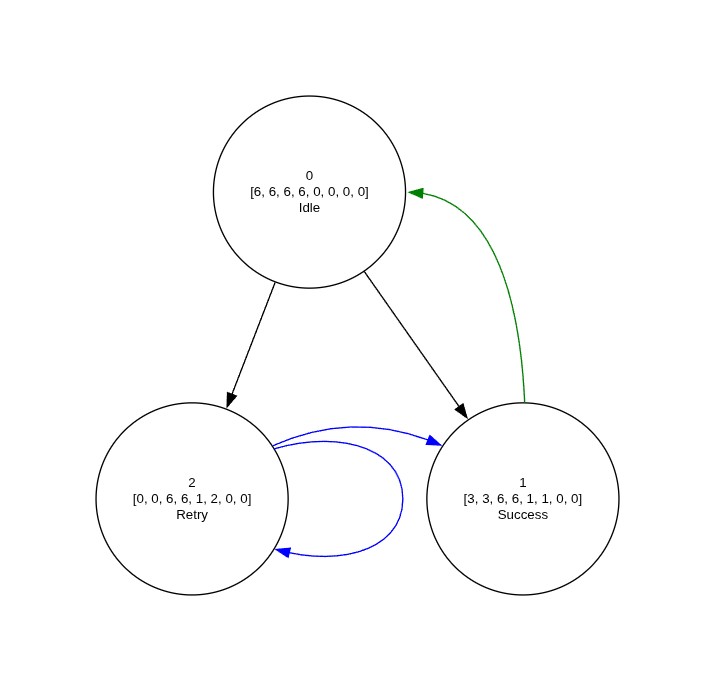
\includegraphics[width=0.75\textwidth]{figures/thinkteam11.png}
	\caption{Generated state space for the modified ThinkTeam protocol}
	\label{fig:thinkteam-snippet}
\end{figure}

\paragraph{Discussion of the Results} 

The experimental results for the Modified ThinkTeam Protocol, shown in Table~\ref{tab:thinkteam_results}, are consistent with the expected behavior of the \textsc{ARIA} exploration engine and provide empirical support for the correctness of the generated state spaces.
\begin{table}[ht]
	\centering
	\caption{Experimental Results for the Modified ThinkTeam Protocol}
	\label{tab:thinkteam_results}
	% Wir definieren einen zentrierten X-Spaltentyp:
	\newcolumntype{Y}{>{\centering\arraybackslash}X}
	
	\begin{tabularx}{\textwidth}{c Y Y Y }
		\toprule
		\textbf{Users ($n$)} & \textbf{States} & \textbf{Transitions} & \textbf{Avg. Time [s]}  \\ 
		\midrule
		1 & 3 & 5  & 0.0047 \\
		2 & 5 & 10 & 0.0049  \\
		3 & 7 & 15 & 0.0052  \\ 
		50 & 101 & 250 & 0.0088\\
		100 & 201 & 500 & 0.0132\\
		500 & 1001 & 2500 & 0.1415 \\
		\bottomrule
	\end{tabularx}
\end{table}

The observed linear growth of the state space ($2n+1$) and the transition count ($5n$) is consistent with the expected theoretical complexity of the protocol. This suggests that the exploration engine handles the interleaving of concurrent request paths in a systematic manner while preserving the intended mutual exclusion behavior of the document vault. The fact that the same structural pattern remains visible even for $n=500$ roles further indicates that the interaction rules scale robustly for this class of examples.

A central challenge in translating choreographies into explicit state spaces is the consistent management of local instruction pointers. The results are consistent with the assumption that \textsc{ARIA} updates the program counters of both the \texttt{Checkout} role and the corresponding \texttt{User[i]} processes coherently during interactions. This includes recursive continuations from \texttt{Success} back to \texttt{InitialAccess} as well as transitions into the \texttt{RetryPhase}. Moreover, the absence of unexpected state growth suggests that no spurious intermediate states are introduced during exploration.

Together, these observations suggest that the generated state space provides a suitable basis for later probabilistic analyses once concrete values are assigned to the symbolic rates $\lambda$, $\theta$, and $\mu$.

The low runtime, including $0.1415$ seconds for 500 users, suggests that for protocols with relatively low coupling, the overhead of exploration remains modest.

\subsection{Peer-to-Peer Protocol}
\label{sec:p2p}

The Peer-to-Peer (P2P)\footnote{https://www.prismmodelchecker.org/casestudies/peer2peer.php} protocol models a decentralized network in which multiple peers exchange data blocks without a central coordinator. From the perspective of state-space exploration, it constitutes a representative example of a highly concurrent system with substantial interleaving and rapid combinatorial growth.

\paragraph{Benchmark Objective: Interleaving, State-Space Explosion, and Emerging I/O Bottlenecks}
In contrast to the modified ThinkTeam protocol, which primarily serves as a compact benchmark for cyclic coordination and retrial behavior, the P2P case study is intended to stress the exploration engine under conditions of extreme concurrency. Its main purpose is therefore to evaluate whether the implementation handles the interleaving of many independently progressing participants correctly and whether it remains robust in the presence of severe state-space explosion.

Due to the large number of peers and the relative independence of their local actions, the protocol induces a very high number of reachable configurations. This makes it a suitable benchmark for testing the correctness of the interleaving logic, the robustness of state deduplication, and the practical scalability of the overall exploration procedure.

At the same time, this case study revealed an additional practical limitation during development and testing. While the exploration itself remained efficient, the explicit serialization of the generated transition structure introduced substantial storage demands. The P2P benchmark therefore also became a useful case for observing how, in large-scale explicit-state generation, the bottleneck may shift from computation to output and storage.

\paragraph{Choreographic Encoding}
As shown in \cref{lst:p2p}, the P2P protocol is encoded using a parametric family of \texttt{Client[i]} roles, where each client maintains a local state describing which data blocks have already been obtained. Concretely, for every client $i \in \{1, \dots, n\}$, the variables \texttt{b[i]1}, \dots, \texttt{b[i]5} record the availability of the corresponding blocks, with value $0$ indicating that a block is not yet available locally and value $1$ indicating that it has been acquired.

The protocol itself is captured by the recursive procedure \texttt{PeerToPeer}. In each execution step, a client performs a local probabilistic action that updates one of its block variables and then recurses back to the same protocol. The five branches shown in the listing correspond to the acquisition of different blocks, each annotated with its own symbolic rate. This encoding abstracts from concrete message-routing details and instead focuses on the stochastic progression of local block acquisition.

From the perspective of state-space exploration, the crucial aspect of this model is that the clients evolve largely independently. Since each \texttt{Client[i]} may perform its next local step without requiring immediate synchronization with the others, the exploration engine must account for a very large number of possible interleavings. Even though the local behavior of an individual client is simple, the combination of parametric roles, recursive continuation, and multiple independently evolving block variables leads to substantial combinatorial growth of the global state space.

This makes the encoding particularly suitable for evaluating whether \textsc{ARIA} can explore large concurrent systems systematically while maintaining a consistent treatment of interleaving and duplicate detection. In this sense, the protocol complements the previous ThinkTeam case study: whereas ThinkTeam emphasizes cyclic coordination and retrial behavior in a comparatively compact state space, the P2P model stresses the exploration engine through massive concurrency and combinatorial growth.

The P2P protocol is the primary benchmark for \textit{RQ 2}. It features a high degree of independence, where multiple peers make local probabilistic decisions about block acquisition. The evaluation focuses on whether the EPP-guided exploration can safely manage the resulting interleavings and the subsequent re-synchronization of these independent local states into a consistent global Markov chain.
\begin{listing}[h]
	\begin{minted}{text}
		preamble
		"ctmc";
		"const int n = 5;"
		endpreamble;
		
		Client[i] -> i in [1...n] Client[i] : "b[i]1 = 0", "b[i]2 = 0" , "b[i]3 = 0", "b[i]4 = 0", "b[i]5 = 0";
		
		{
			PeerToPeer := Client[i] -> Client[i] : 
		   (+["rate1 * 1"] "b[i]1'=1" " " . PeerToPeer
			+["rate2 * 1"] "b[i]2'=1" " " . PeerToPeer
			+["rate3 * 1"] "b[i]3'=1" " " . PeerToPeer
			+["rate4 * 1"] "b[i]4'=1" " " . PeerToPeer
			+["rate5 * 1"] "b[i]5'=1" " " . PeerToPeer)
		}
		
	\end{minted}
	\caption{The Peer-To-Peer Protocol in the specified syntax}
	\label{lst:p2p}
\end{listing}

\paragraph{Discussion of the Results}
\begin{table}[ht]
	\centering
	\begin{threeparttable}
		\caption{Comparison of \textsc{ARIA} and PRISM results for the P2P protocol.}
		\label{tab:p2p_comparison}
		\newcolumntype{Y}{>{\centering\arraybackslash}X}
		
		\begin{tabularx}{\textwidth}{c c Y Y Y Y Y Y}
			\toprule
			\textbf{$n$} & \textbf{$k$} & \textbf{States (ARIA)} & \textbf{States (PRISM)} & \textbf{Transitions (ARIA)} & \textbf{Transitions (PRISM)} & \textbf{Avg. Time [s]} & \textbf{States/s} \\
			\midrule
			4 & 4 & 65{,}536       & 65{,}536       & 1{,}048{,}576   & 524{,}288       & 2.6451   & 24{,}776 \\
			4 & 5 & 1{,}048{,}576  & 1{,}048{,}576  & 20{,}971{,}520  & 10{,}485{,}760  & 46.5617  & 22{,}520 \\
			5 & 4 & 1{,}048{,}576  & 1{,}048{,}576  & 20{,}971{,}520  & 10{,}485{,}760  & 42.6897  & 24{,}564 \\
			5 & 5 & 33{,}554{,}432 & 33{,}554{,}432 & 838{,}860{,}800 & 419{,}430{,}400 & 2343.3567\tnote{*} & 14{,}319 \\
			\bottomrule
		\end{tabularx}
		
		\begin{tablenotes}
			\small
			\item[*] Measured without I/O serialization to disk due to memory limits.
		\end{tablenotes}
	\end{threeparttable}
\end{table}

A comparison with the corresponding PRISM results (see \cref{tab:p2p_comparison}) reveals that the number of reachable states coincides exactly for all evaluated parameter settings. However, the number of transitions generated by \textsc{ARIA} is consistently twice as large as the PRISM count.

This systematic factor of exactly 2.0 is a direct consequence of how self-loops are handled. The state space of the P2P protocol forms a \textit{binary hypercube} of dimension $D = n \times k$, where $n$ denotes the number of peers and $k$ represents the number of data blocks per peer. The total number of reachable states is thus $2^D$. 

In our choreographic encoding (see \cref{lst:p2p}), each peer provides all $k$ acquisition branches in every state. The \textsc{ARIA} exploration engine exhaustively follows every branch defined in the choreography. If a block is not yet possessed, the assignment results in a state change; if the block is already held, the assignment results in a self-loop. Consequently, every state in the \textsc{ARIA} model has exactly $D$ outgoing transitions, leading to a total transition count of $T_{\textsc{ARIA}} = D \cdot 2^D$.

In contrast, PRISM's transition count for CTMCs (specifically in \texttt{.tra} files) typically excludes self-loops, as they do not affect the exit rates or the transient behavior of the Markov chain. PRISM only records the edges of the hypercube where an actual state change occurs. Since a $D$-dimensional binary hypercube has exactly $D \cdot 2^{D-1}$ edges, the resulting ratio is:
\begin{equation}
	\frac{T_{\textsc{ARIA}}}{T_{\text{PRISM}}} = \frac{D \cdot 2^D}{D \cdot 2^{D-1}} = 2
\end{equation}

This observation is important for two reasons. First, the exact agreement in the number of reachable states ($\Delta S = 0$) provides strong empirical support that both tools explore the identical global configuration space. Second, the systematic factor of two indicates that the difference is structural rather than accidental, reflecting a more \textit{semantically exhaustive} representation of the interaction choices in our model. Taken together, these results suggest that \textsc{ARIA} explores interleavings, independent local decisions, and the resulting re-synchronization behavior in a semantically consistent manner.

The measured throughput remains in the range of approximately 22{,}000 to 25{,}000 explored states per second for the smaller configurations and decreases to about 14{,}000 states per second for the largest instance, reflecting the increasing overhead associated with larger state vectors and transition structures.

The declining throughput for larger benchmark instances is consistent with increasing memory pressure during exploration. As the worklist grows and the number of discovered states increases, the implementation must maintain a larger number of live objects simultaneously, including state vectors, worklist entries, and hash-based indexing structures. A plausible consequence is increased heap pressure and additional garbage-collection overhead, which may contribute to the reduced exploration rate. Although no dedicated heap or garbage-collection profiling was performed, the runtime behavior is consistent with this explanation.

For the largest Peer-to-Peer instances, the limiting factor was not only the size of the reachable state space itself, but also the overhead of serializing and storing the generated model. In particular, the output of explicit transition data imposed substantial I/O demands, which became a practical bottleneck alongside memory consumption.
\subsection{Dining Cryptographers Protocol}
\label{sec:dining-cryptographers}

The Dining Cryptographers protocol, originally introduced by Chaum~\cite{Chaum1988}, is a classical benchmark for reasoning about anonymity in distributed systems. The protocol describes a group of cryptographers who wish to determine whether their dinner was paid for by their master or by one of themselves, while preserving the anonymity of the actual payer in the latter case.

The protocol proceeds in two phases. First, each cryptographer flips a private coin and shares its outcome only with the neighbour on the right. Second, each participant announces whether the two visible coin values agree or disagree. If a cryptographer is the payer, however, it announces the opposite result. By evaluating the parity of the public announcements, the group can determine whether the master paid or whether one of the cryptographers paid, without revealing the payer's identity.

\paragraph{Benchmark Objective: Guarded Branching and Conditional Control Flow}
In contrast to the previous case studies, the Dining Cryptographers protocol is particularly useful for evaluating the treatment of conditional control flow. The protocol combines local probabilistic choices with guard-dependent announcements, making it a suitable benchmark for testing whether the exploration engine resolves \texttt{IfThenElse} structures correctly during state-space generation.

Of particular interest is the distinction between balanced and unbalanced conditionals. Depending on the current local observations and on whether a participant is the payer, different control-flow paths become enabled. This makes the protocol well suited for assessing whether the implementation handles both branching cases consistently, excludes blocked continuations correctly from the generated state space, and restores a consistent control-flow alignment when a condition evaluates to false and no explicit \texttt{else} branch is provided.

This protocol specifically addresses \textit{RQ 1}, as it relies heavily on unbalanced conditional flows to model the cryptographers' announcements. It serves as a test case for the semantic rules developed to handle the absence of explicit \texttt{else} branches, ensuring that the exploration engine correctly resynchronizes process control flows even when certain branches are skipped by some participants.

\paragraph{Choreographic Encoding}
In our encoding (see \cref{app:dining-cryptos}), each cryptographer is represented as a separate role with local state variables for the coin value and the final agree/disagree statement. In addition, the model contains a variable identifying the payer. The protocol begins with an initialization step that determines the payer, followed by probabilistic local actions that assign the relevant coin values.

The announcement phase is modeled by guarded transitions whose conditions depend on the local coin value, the neighbouring coin value, and whether the current participant is the payer. As a result, the generated model must combine probabilistic branching, local state updates, and dependency-sensitive guarded control flow in a semantically consistent manner.

For a parameterized system of $N$ cryptographers, the protocol generalizes in the standard way: each participant compares its own coin value with that of its neighbour and publishes either agreement or disagreement, with the payer inverting the expected statement. Collectively, these public announcements determine whether the payer was one of the cryptographers or the master.

\paragraph{Discussion of the Results}
\begin{table}[t]
	\centering
	\caption{Comparison of ARIA and PRISM for the Dining Cryptographers benchmark.}
	\label{tab:dining-comparison}
	\begin{tabularx}{\textwidth}{c|rrr|rrr|rr}
		\hline
		$N$ & \multicolumn{3}{c|}{ARIA} & \multicolumn{3}{c|}{PRISM} & \multicolumn{2}{c}{Difference} \\
		& States & Transitions & Time (s) & States & Transitions & Time (s) & $\Delta S$ & $\Delta T$ \\
		\hline
		3 & 289   & 588    & 0.02999 & 286   & 585    & 0.001 & +3 & +3 \\
		4 & 1736  & 4519   & 0.08096 & 1733  & 4580   & 0.01  & +3 & -61 \\
		5 & 9879  & 32158  & 0.49854 & 9876  & 32315  & 0.03  & +3 & -157 \\
		6 & 54058 & 211185 & 3.21513 & 54055 & 211566 & 0.07  & +3 & -381 \\
		\hline
	\end{tabularx}
\end{table}

\cref{tab:dining-comparison} shows the results of the state-space exploration for the Dining Cryptographers protocol. For all evaluated instances, \textsc{ARIA} constructs exactly three more states than PRISM. This indicates a systematic structural difference between the generated models rather than a random implementation artifact. The number of transitions also differs slightly, although the deviation is not constant across instances: for $N=3$, \textsc{ARIA} generates three additional transitions, whereas for $N \geq 4$ it generates fewer transitions than PRISM.

Overall, the transition counts indicate a systematic but limited discrepancy between the models generated by \textsc{ARIA} and PRISM. In absolute terms, the deviation grows with $N$ ($3$, $61$, $157$, and $381$ transitions for $N=3,\dots,6$), while in relative terms it becomes smaller as the models grow. This suggests that the two constructions remain structurally very close, even though they are not derived from fully equivalent specifications.

A plausible explanation for these differences is that the two models do not encode the protocol in exactly the same way. In particular, the PRISM reference model is formulated as an MDP, whereas the \textsc{ARIA} encoding constructs an explicit state space directly from the choreography. Moreover, the control-flow structure differs slightly: the PRISM model uses local status variables together with explicit enabled commands and a synchronizing \texttt{done} loop, while the choreographic version resolves progress through sequential phases and control-flow resynchronization in the exploration semantics. As a result, both models capture the same protocol behavior at a high level, but they need not induce identical state-transition structures. 

Despite these structural differences, a comparison with established PRISM reference models remains useful for assessing the plausibility of the models generated by \textsc{ARIA}. As widely used representations of the respective protocols, the PRISM models provide a baseline against which the complexity of the generated state spaces can be interpreted. In particular, comparable growth trends as $N$ increases suggest that the choreographic abstraction does not lead to disproportionate additional state-space growth. Such observations do not establish full equivalence, but they do increase confidence that \textsc{ARIA} produces structurally meaningful models that are broadly consistent with established references.
